%
% File acl2016.tex
%
%% Based on the style files for ACL-2015, with some improvements
%%  taken from the NAACL-2016 style
%% Based on the style files for ACL-2014, which were, in turn,
%% Based on the style files for ACL-2013, which were, in turn,
%% Based on the style files for ACL-2012, which were, in turn,
%% based on the style files for ACL-2011, which were, in turn, 
%% based on the style files for ACL-2010, which were, in turn, 
%% based on the style files for ACL-IJCNLP-2009, which were, in turn,
%% based on the style files for EACL-2009 and IJCNLP-2008...

%% Based on the style files for EACL 2006 by 
%%e.agirre@ehu.es or Sergi.Balari@uab.es
%% and that of ACL 08 by Joakim Nivre and Noah Smith

\documentclass[11pt]{article}
\usepackage{acl2016}
\usepackage{times}
\usepackage{url}
\usepackage{latexsym}
\usepackage[hidelinks]{hyperref}
\usepackage{graphicx}
\usepackage{float}
\usepackage{cleveref}
\usepackage{placeins}
\aclfinalcopy % Uncomment this line for the final submission
%\def\aclpaperid{***} %  Enter the acl Paper ID here

%\setlength\titlebox{5cm}
% You can expand the titlebox if you need extra space
% to show all the authors. Please do not make the titlebox
% smaller than 5cm (the original size); we will check this
% in the camera-ready version and ask you to change it back.

\newcommand\BibTeX{B{\sc ib}\TeX}

\title{Building predictors for the game mia}
%nur sichtbar in finaler submission.
\author{Falko Benezan \\
  ID: 3617296\\
  {\tt falko.benezan@}\\
  {\tt student.uni-tuebingen.de} \\\And
  Alexander Diegel \\
	ID: 3980486 \\
  {\tt alexander.diegel@}\\
  {\tt student.uni-tuebingen.de} \\}

\date{}

\begin{document}
\maketitle
\begin{abstract}
  This term paper deals with the topic of predicting different artificial intelligence approaches based on the game mia. It starts with an short introduction to artificial intelligence. Then, the description of the game mia on which the project is based on. Afterwards, the strategies of the different implemented artificial intelligences (AI) are explained. It follows an explanation of our approach predicting the behavior of the different AIs. Finally, the results of the experiments are discussed.
  %TODO weiteres?
\end{abstract}


\section{Introduction}
Artificial intelligence has become an increasingly important field in computer science and other areas such as automotive (self-driving cars) or security (face-detection).
In computer games artificial intelligence reaches new stages of success (Google bot AlphaGo for the game go). In this term paper we now want to answer the question if it is possible to predict different artificial intelligence approaches based on the game mia. The main achievement would be the accuracy of correct predictions if a player (AI) is willing to lie or is telling the correct value of the dice. The question if the actual value is lesser or greater than the called one seems not as important as the prediction of a lie itself. 
%TODO noch mehr?



\section{The Game}
Mia is a simple dice game that is played with two dices and a flat bottomed container (or a dice cup). At the beginning each player has a certain amount of lives (e.g. five).
The first player rolls the dices but keeps their values hidden from the other players. He then can decide if he wants to tell the truth to the next player and announce a value that was actually rolled. Alternatively he can lie and announce a greater or lesser value than the rolled one.
But each player has to announce a greater value than the previous player.
The next player (who still has not seen the actual values) can now believe the passer, call the passer a liar and look on the dice or pass the dice to the next player (still without looking) announcing a higher value. 
A player looses a life if he called the previous one a liar and looked on the values to find out that they are what the previous player has announced or even higher. Otherwise the previous player looses a life. 
The higher value of the roll is multiplied by ten and then added to the other die (a 4 and a 2 is 42). 
The \textbf{scoring} is from highest to lowest:  21 (Mia), 66, 55, 44, 33, 22, 11, 65, 64, 63, 62, 61, 54, 53, 52, 51, 43, 42, 41, 32, 31.
If a player announces mia the next player either believes him, give up (without looking at the dices) and looses one life. Or he may look at the dice. If it was actually mia then he looses two lives if it was not, the previous player looses a life. (For further information see \cite{mia:2016}.)

\section{Implementation of the Game}
For the implementation we use C++ and Qt to build the GUI-Application, as IDE we used Qt-Creator. To implement an artificial intelligence according to the support vector machine learner we used the OpenCV library.
The ingame AI is used to distinguish between lies and the truth of announced values.
For the prediction we used the last announced value, the actual value and an indicator to show the start of a new game. 
To train the SVM we additionally used an indicator if the actual (value that previous player announced) value was a lie.\\
The difference between the strategy for liar detection and gameplay  follows in \cref{sec:setstrat}.

\section{Setup and Strategies}
\label{sec:setstrat}
To measure the performance of the predictor different artificial intelligence approaches were used. For data acquisition we used a homogeneous set of players in our game implementation and let it generate game data. 
Therefore the output of one AI is the input of the following AI in the game.
For each turn we reported:
\begin{itemize}
	\item player number
	\item previous player number
	\item if the turn is the first one in the round (new game)
	\item new announced value
	\item actual rolled value
	\item previous announced value
	\item does the player look onto the dices or not
\end{itemize}
Since the actual rolled value is mostly hidden from the players. We decided to learn the predictor the players strategies only based on: new game, last announced value and new announced value (this seems most realistic).
We then create liar labels for the datasets due to comparison of the new announced value and the actual rolled value for training purposes.
Each dataset is split up to training data and test data. So we train the predictor for the different approaches by using cross validation (determination of parameter C) on the training data and measure the performance (generalization) on the test data. The test set is 30 percent of the data set, the others are training data.
In the end we will compare the results of the implemented AIs detecting lies by taking the indicator that the ingame AI will look at the values (saying the former player was a lier) and the predictions of our predictor (see \cref{secDiscussionOfResults}).

We examined three different types of artificial intelligence approaches. First the statistical approach where the AI acts very straight forward. Then an AI with a certain degree of randomness in its call and look behavior. At the end we implemented a learning AI with different calling behaviors to examine if the predictor is able to learn the strategy of a learning player. Last we wanted to know how many samples it takes until there is convergence of accuracy in the predictor. 

\subsection{Statistic Approach}
\label{ssec:statistic}
\Cref{tbl:stat1} shows basic statistic probabilities of the game mia. Note: if the value (call/announcement of previous player) is 21 then the current player can either look up the dices and possibly looses two lives or he can save himself by rolling a 21 as well. 

\begin{table}[H]
	\centering
	\small 
	\begin{tabular}{|c|c|c|c|c|c|c|c|}
		\hline 
		Value&31&32&41&42&43&51&52\\ \hline
		\%&94&89&83&78&72&67&61\\ \hline 
		&&&&&&& \\ \hline
		Value&53&54&61&62&63&64&65\\ \hline
		\%&56&50&44&39&33&28&22\\ \hline 
		&&&&&&& \\ \hline
		Value&11&22&33&44&55&66&21\\ \hline
		\%&19&17&14&11&8&6&6 \\ \hline
				
	\end{tabular}
	\caption{Shows the probability of getting a higher dice result than the announced value.}
	\label{tbl:stat1}
\end{table}

The artificial intelligence based on the statistical approach is quite easy. It calls a the previous player a liar if the probability of lying is greater than the probability to say the truth.
This AI always says the truth if possible, otherwise it take a random value greater than the last announced value.


\subsection{Approach with certain degree of randomness (Primitive Random)}
\label{ssec:primitive}
This AI will call with a certain probability a value that is greater than the actual rolled value if the value is lower than the one of the previous player. Also the AI will look on the dices with a probability that arises with decreasing beat probability (see \cref{tbl:stat1}) of a announced value (a 31 will not be looked at with probability near 100 percent, 21 is looked at with 100 percent). This AI always says the truth if it is possible (meaning the rolled value is greater than the last announced value). Otherwise this AI will call a random value.

\subsection{A SVM learning approach}
The next step was to create a new type of artificial intelligence that changes its behavior during the history/time of the game.
Therefore, we used a SVM implementation with different behavior by calling a value (meaning lie or tell the truth).

\subsubsection{SVM variant 1}
\label{sssec:svm1}
This variant of the AI says the truth or uses the next possible value greater than the last announced one.

\subsubsection{SVM variant 2}
\label{sssec:svm2}
This AI variant always says the truth if it is possible or calls a random value greater than the last announced one. 

\subsubsection{SVM variant 3}
\label{sssec:svm3}
This AI always calls a possible random value that is independent from the actual rolled dice value.

\subsubsection{SVM variant 4}
\label{sssec:svm4}
This AI always announces a lower or equal value than the actual rolled value if it is possible. Otherwise it uses a random value greater than the last announced one. This AI is willing to lie whenever it is possible. 

\section{The Predictor}
To predict the different strategical approaches we used a support vector machine (SVM) predictor with radial basis functions. A linear predictor would not have been sufficient due to the complexity of data, but with the SVM-predictor adequate results could be expected.
By using SVM we are interested in separating two (or more) classes by a separating hyperplane with maximal margin. The margin is defined with respect to the training points as the minimal distance between the hyperplane and a training point.(See \cite[187--227]{Schoellkopf:02}.)

\section{Discussion of Results}
\label{secDiscussionOfResults}
An overview of the maintained results can be seen in \cref{tab:results}.
In all but one case the learned predictor was able to predict the lier labels better than the AIs. Moreover we can conclude that the predictor was able to learn the strategy of the different approaches quite well. 

\begin{table}[H]
\centering
\small
\begin{tabular}{|l|l|l|l|l|}
\hline
\textbf{strategy}&\textbf{sdetect}&\textbf{C}&\textbf{pdetect} \\ \hline
\textbf{statistic}&\textbf{0.473}&\textbf{0.0001}&\textbf{0.863} \\ \hline
\textbf{primitive}&\textbf{0.585}&\textbf{0.5}&\textbf{0.849} \\ \hline
\textbf{SVM1}&\textbf{0.964}&\textbf{2.0}&\textbf{0.971} \\ \hline
\textbf{SVM2}&\textbf{0.810}&\textbf{0.6}&\textbf{0.797}\\ \hline 
\textbf{SVM3}&\textbf{0.844}&\textbf{3.0}&\textbf{0.971}\\ \hline 
\textbf{SVM4}&\textbf{0.642}&\textbf{2.0}&\textbf{0.989} \\ \hline
\end{tabular}
\caption{Obtained results in the experiments. Strategy, strategies liar detection (sdetect), parameter C for predictor, predictors liar detection (pdetect) on test data. The predictor is a python SVM implementation.}
\label{tab:results}
\end{table}

The artificial intelligence based on the statistic approach (see \cref{ssec:statistic}) has the worst results of all our experiments. Our predictor was able to achieve a result of 86\% and more or less learn the AIs strategy.
The approach with a certain degree of randomness (see \cref{ssec:primitive}) was able to detect around 60\% (the predictor again beat the ingame AI and was able to learn their strategy).
The learning of the SVM helps to improve the ingame predictions and learn the strategy of the other players (the ingame results are quite as good as the our predictor implemented in python).
Summing up we can say that the ingame AIs results are the better the less randomness exist in the calling behavior of the other players.
The predictor was able to learn nearly all strategies good.
The following convergences consider the convergence of the python predictor not the ingame AI convergence.

For the statistical approach convergence takes place around 4000 samples if we allow one percent of deviation in both directions (see \cref{fig:conv_stat}). 
In \cref{fig:conv_prim} the convergence can be seen more easily. It is again about 4000 samples. Afterwards there is only little variation of the accuracy. 
For the SVM approaches can be seen that variant 1 and variant 3 converge to the same value of accuracy (0.97). Convergence for both variants is about 2000 samples. Variant 2 of the SVM approach has a lower level of accuracy meaning that this one is harder to predict correctly than the others (under the given data). The convergence of variant 2 is at around 3000 samples. Variant 4 has the highest rate of accuracy with 98 percent and converges about 2500 samples (compare \cref{fig:conv_svmall}).

Comparing the convergence of the ingame AI (\cref{fig:conv_ingameSVM1}) and the python predictor (\cref{fig:svm1}) we can say that both converge near to 1500 samples. 
The strategy of a lier has been detected by both ingame and python predictor. 

\Cref{fig:svm1,fig:svm2,fig:svm3,fig:svm4} show the classification of the ingame artificial intelligence based on the SVM learner.
The green color represents values that are going to be accepted as the truth by other players. Blue areas represent that the actual value is detected as a lie.
On the horizontal axis there is the actual value. On the vertical axis there is the last value \footnote{The axis are in numerical order. Therefore, non valid dice values for the mia game are represented.}. 
On the left half the running game is represented and on the right side new game predictions are depicted. The origin of the image is on the top left side. 

\begin{figure}[H]
	\centering
	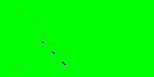
\includegraphics[width=.45\textwidth]{../testdata/svm1.png}
	\caption{Classification of SVM-AI variant 1.}
	\label{fig:svm1}
\end{figure}

\Cref{fig:svm1} shows that the SVM-AI (see \cref{sssec:svm1}) can learn the calling strategy of saying the next greater value. The blue points show that the next greater value is quite often a simple lie.

\begin{figure}[H]
	\centering
	
\includegraphics[width=.45\textwidth]{../testdata/svm2.png}
	\caption{Classification of SVM-AI variant 2}
	\label{fig:svm2}
\end{figure}

\Cref{fig:svm2} has a green area between the blue dots. That is because the values around 31 and 42 are often true and the AI accepts this calls (see \cref{sssec:svm2}).

\begin{figure}[H]
	\centering
	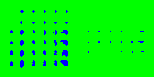
\includegraphics[width=.45\textwidth]{../testdata/svm3.png}
	\caption{Classification of SVM-AI variant 1}
	\label{fig:svm3}
\end{figure}
In \cref{fig:svm3} you can see clearly that the variance of the liars classification increases due to the random calling procedure of the third variant (see \cref{sssec:svm3}). And since the AI is likely to lie there are blue points on the right side of the image, meaning that start values are considered to be likely a lie. 

\begin{figure}[H]
	\centering
	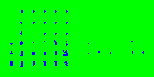
\includegraphics[width=.45\textwidth]{../testdata/svm4.png}
	\caption{Classification of SVM-AI variant 1}
	\label{fig:svm4}
\end{figure}

In \cref{fig:svm4} where the calling behavior is to say a smaller value (see \cref{sssec:svm4}) if possible the variance of the lier calling is a bit smaller than in \cref{sssec:svm3}.


\FloatBarrier
\section{Supplemental Material}

\begin{figure}[H]
	\centering
	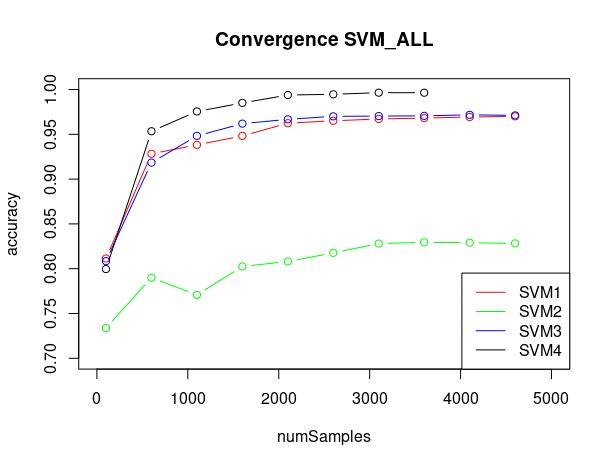
\includegraphics[width=.45\textwidth]{../testdata/convergence_all.png}
	\caption{Comparison of predictor based on all four SVM variants data sets.}
	\label{fig:conv_svmall}
\end{figure}

\begin{figure}[H]
	\centering
	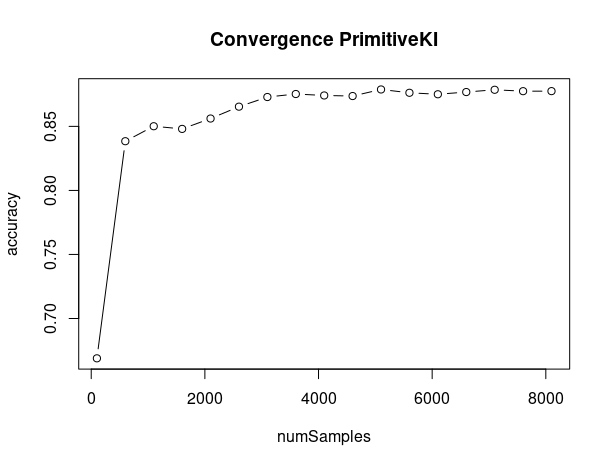
\includegraphics[width=.45\textwidth]{../testdata/conv_prim.png}
	\caption{Convergence of the python predictor on data generated by the approach with certain degree of randomness.}
	\label{fig:conv_prim}
\end{figure}
\begin{figure}[H]
	\centering
	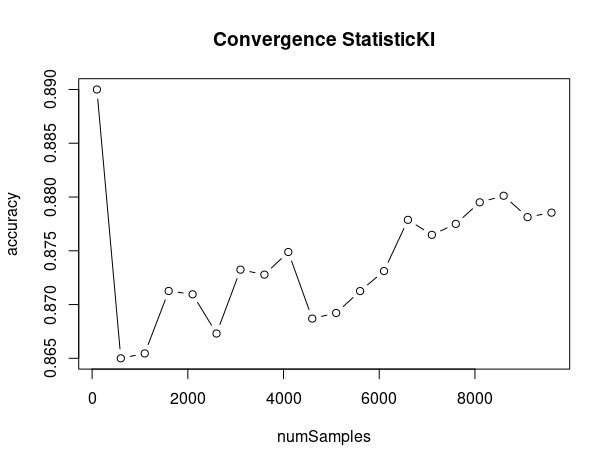
\includegraphics[width=.45\textwidth]{../testdata/conv_stat.png}
	\caption{Convergence of python predictor on data generated by the statistical approach.}
	\label{fig:conv_stat}
\end{figure}

\begin{figure}[H]
	\centering
	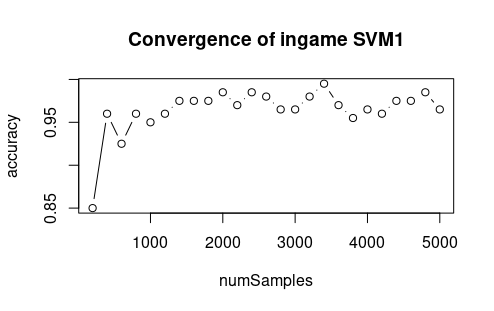
\includegraphics[width=.45\textwidth]{../testdata/conv_ingameSVM1.png}
	\caption{Convergence of the ingame SVM in variant 1.}
	\label{fig:conv_ingameSVM1}
\end{figure}
%10000 for stat und prim
%5000 for svms

%\begin{table}
%\centering
%\small
%\begin{tabular}{cc}
%\begin{tabular}{|l|l|}
%\hline
%{\bf Command} & {\bf Output}\\\hline
%\verb|{\"a}| & {\"a} \\
%\verb|{\^e}| & {\^e} \\
%\verb|{\`i}| & {\`i} \\ 
%\verb|{\.I}| & {\.I} \\ 
%\verb|{\o}| & {\o} \\
%\verb|{\'u}| & {\'u}  \\ 
%\verb|{\aa}| & {\aa}  \\\hline
%\end{tabular} & 
%\begin{tabular}{|l|l|}
%\hline
%{\bf Command} & {\bf  Output}\\\hline
%\verb|{\c c}| & {\c c} \\ 
%\verb|{\u g}| & {\u g} \\ 
%\verb|{\l}| & {\l} \\ 
%\verb|{\~n}| & {\~n} \\ 
%\verb|{\H o}| & {\H o} \\ 
%\verb|{\v r}| & {\v r} \\ 
%\verb|{\ss}| & {\ss} \\\hline
%\end{tabular}
%\end{tabular}
%\caption{Example commands for accented characters, to be used in, e.g., \BibTeX\ names.}\label{tab:accents}
%\end{table}



%\penalty -5000

%We suggest that instead of
%\begin{quote}
%  ``\cite{Gusfield:97} showed that ...''
%\end{quote}
%you use
%\begin{quote}
%``Gusfield \shortcite{Gusfield:97}   showed that ...''
%\end{quote}



%
%\section*{Acknowledgments}
%
%The acknowledgments should go immediately before the references.  Do
%not number the acknowledgments section. Do not include this section
%when submitting your paper for review.

% include your own bib file like this:
%\bibliographystyle{acl}
%\bibliography{acl2016}
\bibliography{acl2016}
\bibliographystyle{acl2016}
\appendix

%\section{Supplemental Material}
%\label{sec:supplemental}
%ACL 2016 also encourages the submission of supplementary material
%to report preprocessing decisions, model parameters, and other details
%necessary for the replication of the experiments reported in the 
%paper. Seemingly small preprocessing decisions can sometimes make
%a large difference in performance, so it is crucial to record such
%decisions to precisely characterize state-of-the-art methods.
%
%Nonetheless, supplementary material should be supplementary (rather
%than central) to the paper. It may include explanations or details
%of proofs or deriations that do not fit into the paper, lists of
%features or feature tempates, sample inputs and outputs for a system,
%pseudo-code or source code, and data. (Source code and data should
%be separate uploads, rather than part of the paper).
%
%The paper should not rely on the supplementary material: while the paper
%may refer to and cite the supplementary material will be available to the
%reviewers, they will not be asked to review the
%supplementary material.
%
%Appendices (i.e. supplementary material in the form of proofs, tables,
%or pseudo-code) should come after the references, as shown here. Use
%\verb|\appendix| before any appendix section to switch the section
%numbering over to letters.


\end{document}
